\section*{Ejercicio 1}

\ejercicio{Crear un fichero ordenacion.cpp con el programa completo
  para realizar una ejecución del algoritmo.}

\begin{flushleft}
  La eficiencia teórica de la función es $O(n^2)$. A modo de práctica
  se intentó calcular el polinomio que da dicha complejitud obteniendo
  como resultado:

  \[
    8.5n^2 -6n + 4.5
  \]

  Dicha aproximación teórica nos da una idea de la forma que pueden
  tener nuestros datos cuando los representemos enfrentando tamaño del
  problema contra tiempo de ejecución, aunque lo que más nos interesa
  conocer es que es un polinomio de segundo grado.
\end{flushleft}

\ejercicio{Crear un script en C-Shell que
  permite ejecutar varias veces el programa anterior y generar un
  fichero con los datos obtenidos.}

\begin{flushleft}
  El script de bash utilizado para realizar la recogida de datos ha
  sido el siguiene:
\end{flushleft}
\newpage
\begin{verbatim}
#!/bin/bash
inicio=100
fin="$4"
incremento="$3"
ejecutable="$1"
salida="$2"

echo "ejecutable: $ejecutable"
echo "salida: $salida"
echo "incremento: $incremento"
echo "fin: $fin"

i=$inicio

while [ $i -lt $fin ]
do
    echo "Ejecutando tam = $i"
    echo `./$ejecutable $i $fin` >> $salida
    ((i+=incremento))
done

\end{verbatim}

\ejercicio{Usar gnuplot para dibujar los datos obtenidos en el
  apartado previo.}

\begin{figure}[H]
  \centering
  \caption{Eficiencia empírica}
  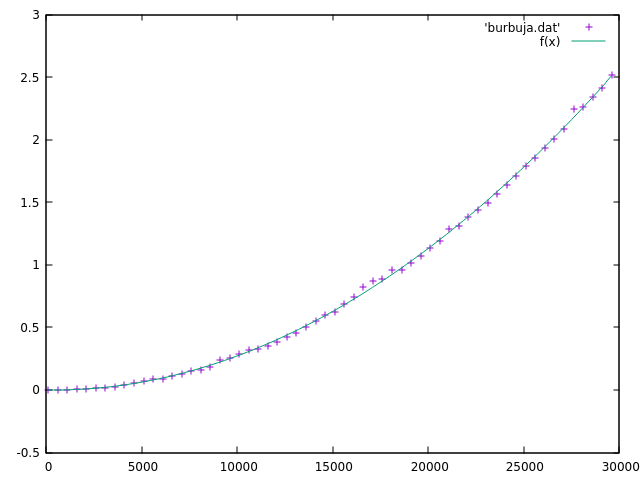
\includegraphics[width=0.8\textwidth]{ejer1/comparacion.png}
\end{figure}